% statistics_and_probability:x07 GDC:NO
\begin{question}
  \hspace*{\fill} [Note maximale: 7]\par
  \medskip

  \noindent Le diagramme de Venn ci-dessous représente les événements A et B où $P(A) = 0,3$ ,\par
  
  \noindent $P(A \cup B) = 0,6 $ et $P(A \cap B) = 0,1$. Les valeurs m , n , p et q sont des probabilités. \par

  \medskip

  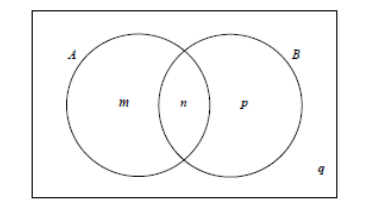
\includegraphics[scale=0.7]{venn_a_b}\par  
  \medskip
  

  (a)\par
  \hspace{2em}(i)  Donnez la valeur de n .\par
  \hspace{2em}(ii) Trouvez la valeur de m , de p et de q .\hspace*{\fill} [4]\par
  
  \medskip

  
  (b) Trouvez $P(B)$.\hspace*{\fill} [2]\par
  
\end{question}

